\documentclass[runningheads]{llncs}
\usepackage{tikz}
\usetikzlibrary{patterns,backgrounds,patterns.meta,shapes.geometric}
\usepackage{pgfplots}

\begin{document}

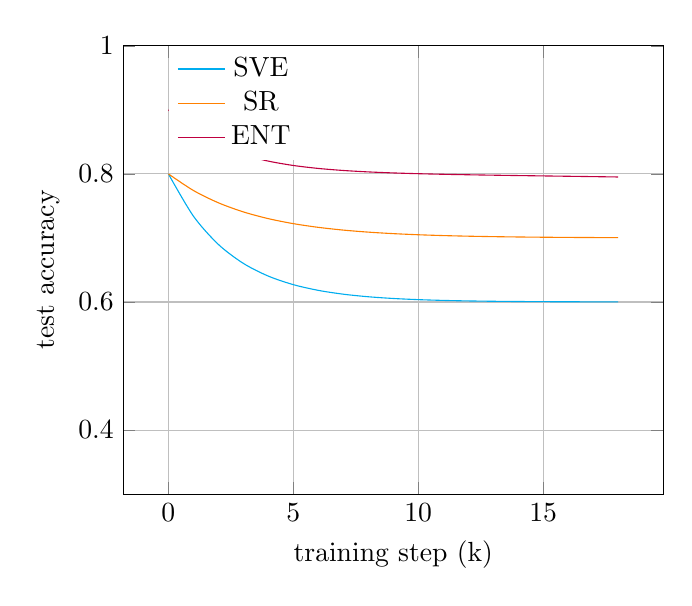
\begin{tikzpicture}[scale=1]
        \begin{axis}[ymin=0.3,ymax=1,
                     xlabel={training step (k)},
                     ylabel={test accuracy},
                     legend pos=south east,
                     grid=major,
                     legend style={at={(axis cs:0,1)},anchor=north west,draw=none}]
            \addplot[smooth,color=cyan,mark=none,domain=0:18,samples=19] {0.6+0.2*exp(-0.4*x)};
            \addplot[smooth,color=orange,mark=none,domain=0:18,samples=19] {0.7+0.1*exp(-0.3*x)};
            \addplot[smooth,color=purple,mark=none,domain=0:18,samples=19] {0.7+0.1*exp(-0.4*x)+0.1*cos(x)};
            \legend{{SVE},{SR},{ENT}};
        \end{axis}
    \end{tikzpicture}

\end{document}